\section{Prozessfluss und allgemeiner Ablauf}
\label{sec:prozessfluss}
Die beiden Event-Logs bilden je einen Genehmigungsprozess für Reisen und deren Kostenabdeckung ab, unterscheiden sich jedoch im konkreten Ablauf.
Nach Tabelle \ref{tab:basisstatistik} und \ref{fig:eventtypes} kommen 17 bzw. 34 verschiedene Ereignisse vor, wobei die Vereinigungsmenge eine Mächtigkeit von 37 beträgt.
Mit menschlicher Sicht werden schnell bestimmte Eventgruppen sichtbar, die inhaltlich zusammengehören (z.B. Trip-Events, Permit-Events), oder auch Muster in der Benennung des concept:name erkennbar.
Um dies maschinell zu untersuchen, werden die 37 Eventnamen als Text mit Python verarbeitet.
Dafür werden die Eventnamen zu Wortlisten anhand des Leerzeichens zerlegt und anschließend Cluster gebildet anhand aller verwendeten Wörter und der Menge der Übereinstimmungen zwischen zwei Namen.
25 Cluster konnten so identifiziert werden, mit Elementanzahlen von 1 bis 34.
Für die einzelnen Cluster wird ein Pattern automatisiert identifiziert, der alle Elemente des Clusters beschreibt.
Cluster mit leeren Patterns oder einem 'allMatch'-Ausdruck wurden verworfen, da sie keine inhaltliche Aussagekraft besitzen.
Mithilfe des 'Algorithmus X' von Donald Knuth \todo{Quelle} wird ein Exact-Cover-Problem der Cluster angegangen und damit Clustermengen identifiziert, bei denen jedes der 37 Events genau einmal eindeutig identifiziert und somit einem Cluster zugeordnet wird.
Es entstehen 12 übrige Filterfunktionen, um jedes Event einer eindeutigen Äquivalenzklasse zuzuordnen.
\begin{wrapfigure}{r}{0.5\textwidth}
    \centering
    \vspace{-0.7cm}
    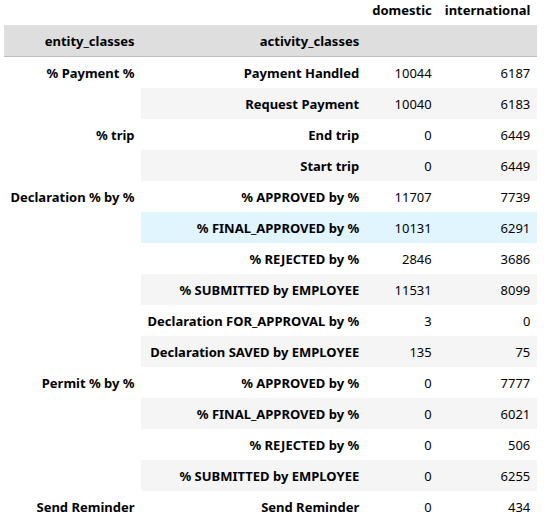
\includegraphics[width=0.5\textwidth]{figures/python/filters}
    \caption{Eventeinteilung je Log nach Filterfunktionen unter Angabe des zugehörigen Patterns}
    \label{fig:filters}
\end{wrapfigure}
Die inhaltliche Bedeutung dieser Relationen wird mit Domänenwissen menschlich interpretiert, sodass Relationen mit Zusammenfassungen durch 'contains-By'-Pattern oder durch das Mischen von Aktivitäten und deren Kontext (z.B. 'Start' und 'Permit' in der gleichen Filterfunktion) entfernt werden, da sie Bedeutungsbereiche vermischen.
Übrig bleiben 2 Filterfunktionen, die Eventnamen inhaltlich einteilen und die Interpretierung von Prozessen unterstützen:
\begin{itemize}
    \item Filterfunktion 'entity\_classes': [DECLARATION, PERMIT, PAYMENT, TRIP, REMINDER SEND]
    \item Filterfunktion 'activity\_classes': [REJECTED, APPROVED, FINAL\_APPROVED, FOR\_APPROVAL, SUBMITTED, END, HANDLED, REMINDER SEND, REQUEST, SAVED, START]
\end{itemize}
% Umfang: 2-3 Seiten
% Assignment-Frage 1: Describe and visualize the general underlying process flow.
%   Reasonable level of abstraction. BPMN / Petri Nets.
% Assignment-Frage 7 (teilweise): Unterschiede International vs. Domestic.
% Quellen: Process Discovery \parencite{leemans_discovering_2013,augusto_automated_2019},
%          BPMN \parencite{dumas_fundamentals_2018}

\subsection{Domestic Declarations}
\label{sec:prozessfluss_domestic}
Bereits absehbar an Abb. \ref{fig:filters} ist, dass im Domestic-Log die Eventgruppen 'Permit', 'Trip' und 'Reminder Send' nicht vorkommen, sodass die Prozessidentifikation sich auf Declaration- und Payment-Aktivitäten konzentrieren kann.
\begin{wrapfigure}{r}{0.55\textwidth}
    \centering
    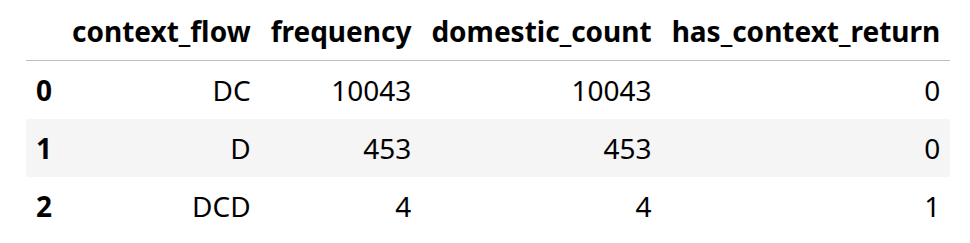
\includegraphics[width=0.55\textwidth]{figures/python/DomesticClasses}
    \caption{Entitätsklassenablauf im Domestic-Log (D=Declaration, C=Payment)}
    \label{fig:domesticclasses}
\end{wrapfigure}
Mithilfe der Filterfunktion 'entity\_classes' und Beschränkungen auf Klassenwechseln wird ersichtlich, dass die Payment-Aktivitäten im Domestic-Log immer gebündelt und nie zu Beginn stattfinden (s. Abb. \ref{fig:domesticclasses}) - in nur 4 der 10500 Fälle wird eine Declaration-Aktion noch erneut nach dem Payment durchgeführt.

% Celonis-Notizen:
%   Cases: 4618 happy path, 10500 total (43,98 %)
%   Happy-Path-TPT: 9 d
%   Algorithmischer Happy Path:
%     Declaration SUBMITTED by EMPLOYEE -> Declaration APPROVED by ADMINISTRATION
%     -> Declaration FINAL_APPROVED by SUPERVISOR -> Request Payment -> Payment Handled
%   Varianten: 100
% Abbildung: BPMN-Export aus Celonis (resources/CelonisDomesticDeclarations.bpmn
%            -> als PDF/PNG nach figures/celonis/ exportieren)

\todo{Abbildung BPMN Domestic (figures/celonis/) und Beschreibung}

\subsection{International Declarations}
\label{sec:prozessfluss_international}

% Celonis-Notizen:
%   Cases: 1369 happy path, 6449 total (21,23 %)
%   Happy-Path-TPT: 66 d
%   Algorithmischer Happy Path:
%     Permit SUBMITTED by EMPLOYEE -> Permit APPROVED by ADMINISTRATION
%     -> Permit FINAL_APPROVED by SUPERVISOR -> Start trip -> End trip
%     -> Declaration SUBMITTED by EMPLOYEE -> Declaration APPROVED by ADMINISTRATION
%     -> Declaration FINAL_APPROVED by SUPERVISOR -> Request Payment -> Payment Handled
%   Varianten: 756
% Abbildung: BPMN-Export aus Celonis (resources/CelonisInternationalDeclarations.bpmn)

\todo{Abbildung BPMN International (figures/celonis/) und Beschreibung}

\subsection{Abstraktionsniveau und Vergleich}
\label{sec:prozessfluss_vergleich}

% - Abstraktion begründen: Varianten-Abdeckung (Top-n-Varianten = x % der Cases),
%   Frequenzfilter im Process Explorer.
% - International = Domestic-Kern + vorgelagerte Permit-Phase + Trip-Events.
% - Optional: Inductive-Miner-Modell aus PM4Py (Jesco, figures/python/) gegenüberstellen.

\todo{Vergleich Domestic vs. International; ggf. PM4Py-Modell von Jesco}
